% Target: 20ish pages total; 13 pages of text, 7 pages of images
\chapter{Load Balancers and Their Placement}
In this chapter we describe our chosen approach for improving the performance of network bound workloads in serverless edge computing environments. We start by explaining our considerations when developing our approach in the context of a serverless edge computing system, and showing in what way our solution changes the system. From there we go into detail about how the load balancing mechanism of our solution works, how it is different from the currently employed methods, and how the choices made in regard to the load balancing method inform other parts of the proposed approach.
Lastly we go into our approach to scaling and scheduling load balancers among the nodes present in the serverless edge computing system. We make use of osmotic scaling and scheduling, a method previously outlined in existing literature. Using this idea of osmotic scaling and scheduling, we provide a concrete implementation of such an approach for placing and deciding on the number of load balancers in the system. The implementation is designed with current state of the art systems such as Kubernetes as the basis, and can thus be used as a reference implementation for use outside of a simulation context. The approach also addresses the challenges of edge computing environments that make current approaches, developed with the cloud in mind, unsuitable. Specifically our approach addresses issues of location awareness, device and network heterogeneity, and dynamically changing workload conditions.
% Target: 2ish pages \w graphics
\section{Concept}
% Note: mention that in our context load balancing and entry-gateway are sort of equivalent. Show their relation a bit
% Note: Mention that our approach uses the method of using real-life experiments to inform simulation

To understand the approach we first take a step back to view the boarder technical context the solution addresses and is built around.
As previously outlined, our solution aims to improve the performance of network bound workloads.
In the context of serverless edge computing systems network bound workloads are characterized by the network being the main or a significant contributing factor to the overall response time.
\begin{figure}
    \centering
    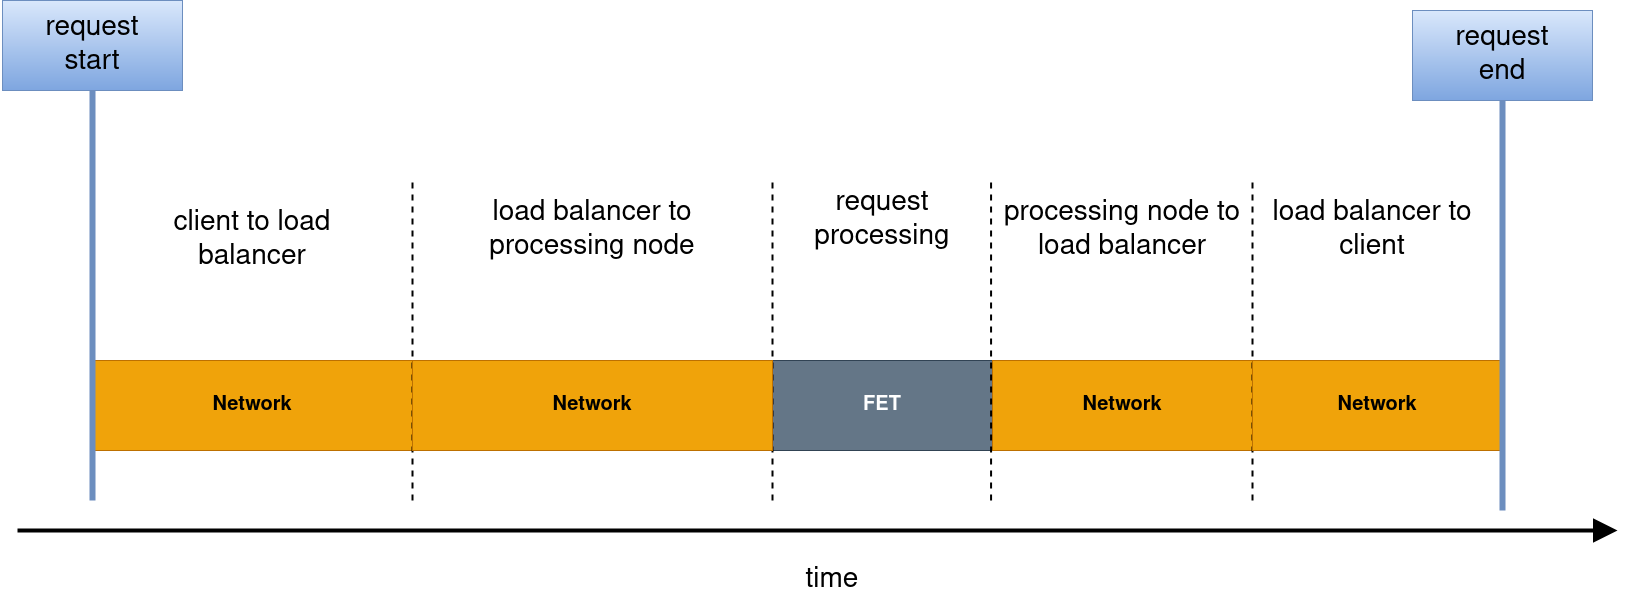
\includegraphics[width=14cm]{graphics/diagrams/request_overview.png}
    \caption{A generic view of the different parts that make up the total request processing time from the perspective of our approach}
    \label{fig:request_net_fet_overview}
\end{figure}
In Figure \ref{fig:request_net_fet_overview} we can see the different processing steps we consider for a request.
A network bound workload in this sense is one where the time taken up by the network portion of handling the request is proportionally speaking significantly larger than the portion taken by the \gls{fet}.
This is typically the case because either the request contains a lot of data that needs to be transported, or because the \gls{fet} is very short.

The primary way by which our approach improves the response times of network bound workloads is thus by reducing the amount of time spent on the network transfer portion of handling a client request.
While optimizing \glspl{fet} is not the primary objective of our approach, at least from a systems design perspective, it still has the potential to additionally reduce \glspl{fet} compared to current methods.
We consider the structure and makeup of the serverless computing system to be a given factor. As a result our approach aims to reduce network times not by changing the network makeup itself, but by utilizing the existing resources as effectively as possible. From a network-optimization perspective this means that each request should take an optimal path from  the client to the node where the request is ultimately processed. 

\begin{figure}
    \centering
    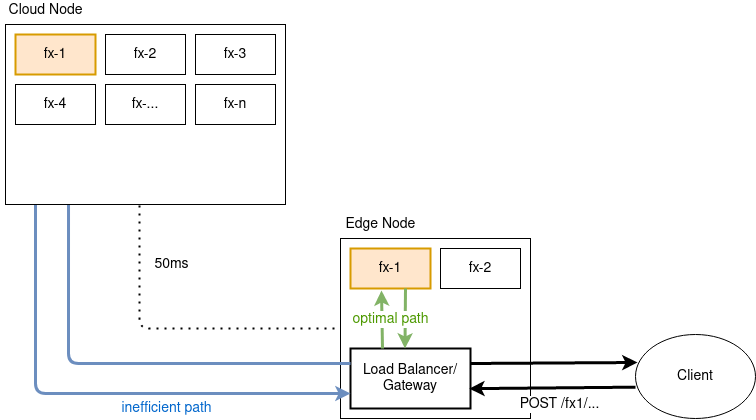
\includegraphics[width=12cm]{graphics/diagrams/efficient_path_example.png}
    \caption{Example diagram showing efficient and inefficient request routing based on network delay. "fx-1" through "fx-2" denote different types of function, and the dotted line denotes a network link between the cloud and edge node with a latency of 50ms}
    \label{fig:efficient_path}
\end{figure}

As can be understood quite intuitively in Figure \ref{fig:efficient_path}, round robin load balancing will in many cases lead to clearly suboptimal choices in terms of incurred network delay. The figure also shows the three key components we consider when trying to make network location based decisions: The client, the load balancer, and the node. Because our approach solely considers application level load balancers, since serverless platforms typically require these for their advanced routing decisions, any given request takes a path from the client to the load balancer, then to the selected upstream node, and back the same way.

Subsequently we want to incur the minimal amount of delay possible from both the hop between the client and load balancer, as well as between the load balancer and upstream node. Our proposed approach handles these two kinds of hops separately, at least for the most part. Since the scope of this work does not include optimizing the location of the serverless function instances themselves, this means we can improve performance through the following methods:
\begin{enumerate}
    \item \textbf{Intelligent load balancing decisions:} load balancers should choose upstream nodes that are both close in the network, and have \glspl{fet} short enough as not to negate the performance won through network proximity
    \item \textbf{Effective placement of load balancers:} the scheduler of the serverless system should place load balancers at locations in the network where they are in close proximity to clients and serverless function instances requested by these clients
    \item \textbf{Efficient scaling of load balancers:} the amount of load balancers should be high enough to provide the needed performance improvement, but not so high that the resources consumed by the load balancers diminish or even negate that effect
\end{enumerate}
In our approach the first method is provided by the load balancer itself. It is continuously updated with information where function instances, typically also referred to as \textit{replicas}, are located. Based on this and other information gathered by the load balancer, it tries to make decisions that lead to faster overall request responsiveness by selecting upstreams that are close and provide fast \glspl{fet}.

The other two methods are handled by the osmotic joint scaling and scheduling component of our approach. While the different methods of improvement are split between these two components of our proposed solution, this does not mean that they are completely separate from each other. Naturally the scheduling and scaling decisions will influence the way in which the placed load balancers work, while these in-turn affect the data gathered for and available to the scaling and scheduling component. The specifics of these two components will be discussed in the next two sections. 

It is also important to note that a significant amount of the approaches' implementation details are not chosen arbitrarily, but are rather the result of continuous cycle of experimentation and evaluation. While not detailed in the approach, the evaluation, result, and discussion chapters of this thesis include some of these experiments, in particular those that give additional insight into the problem domain and yielded results useful beyond informing this specific approach.
% Target: 8 pages with figures
\section{Least Response Time Load Balancing}
In this section we describe the role the load balancer plays in the context of our approach, how it is related to the underlying serverless platform, and the details of how it is implemented.

\subsection{Load Balancing Concepts}
While load balancing might at first appear as a rather simple problem, venturing outside cloud-centric scenarios, where resource homogeneity can be assumed, makes it much more complex of a challenge.
Since we feel the changes implied by resource heterogeneity are often only implicitly covered in literature, or an understanding of the problem is assumed, we believe that it is beneficial to describe it in more detail. This not only helps form a basis on which subsequent research can build, but also gives a lot of contextual information on how our approach relates to the underlying formal problem.

For our formulation of the load balancing problem we consider two types of resources: nodes, and network links. Nodes are the compute nodes in the cluster, and are characterized by the compute capabilities they possess and the function instances they host. Network links are characterized by their latency, and their bandwidth.
\begin{figure}
    \centering
    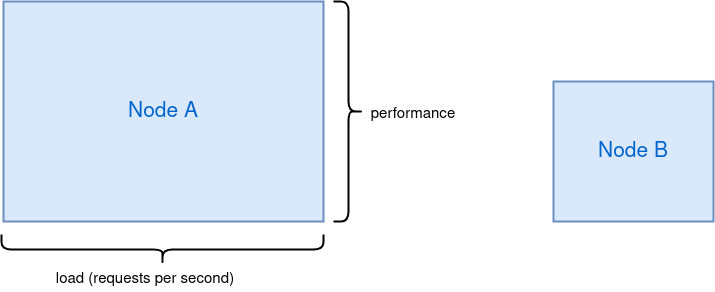
\includegraphics[width=12cm]{graphics/diagrams/load_balancer_squares.png}
    \caption{Rectangles representing a resource in our problem visualization}
    \label{fig:lb_squares_basic}
\end{figure}
To get a more intuitive understanding of the problem we developed a visualization, where resources are depicted as rectangles, where their dimensions correspond to their characterizing attributes. Figure \ref{fig:lb_squares_basic} shows an example of this. The width of the rectangle corresponds to the \textit{load} of the system, in our case measured in \gls{rps}, and the height corresponds to the performance, which since we are concerned about response times is the response time in milliseconds. One should note that, even though maybe counter intuitive, a greater height corresponds to higher performance, which in turn means \textit{lower} response times.
A core concept of this visualization is the capability of resources to \textit{stretch} or \textit{compress}. This means increasing or decreasing width or height of the resource, while doing the inverse to the other side. The condition is that the total area of the resource, i.e. the product of width and height, must be consistent throughout this process. This is effectively the way in which performance regression is modeled in this visualization, but one should not that this way only works under the condition that performance regression is linear with respect to the load. Luckily this is close to observed real world behaviour, %todo cite this
meaning that at least for understanding the underlying problem this visualization holds.
There are, however, limits to this stretching or compressing resources. From a visual perspective there is a bounding box around each resource, which cannot be exceeded in either height or width. This corresponds to the real world behaviour of workloads not getting faster beyond a certain point, even if resources would be available one one side, and requests simply timing out once responses exceed a certain time limit.
\begin{figure}
    \centering
    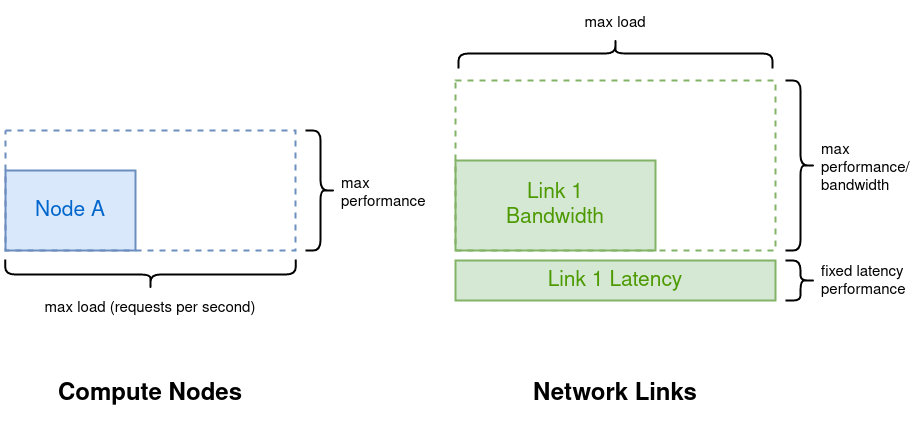
\includegraphics[width=14cm]{graphics/diagrams/lb_squares_real.png}
    \caption{Rectangles representing Node and Network Link resources, including their respective bounding boxes showing maximum load and performance capabilities}
    \label{fig:lb_squares_real}
\end{figure}
Network link resources work slightly differently, as they have a fixed component, dictated by the latency of the link, and a variable component set by the bandwidth. The variable component works as just described, while the static component is constant. Figure \ref{fig:lb_squares_real} shows the variable and static components along with their limits.

Resources can be conditionally linked. This maps the real world conditions of nodes being attached to the cluster via network links. Just like in actual clusters multiple nodes can be dependent on the same network link, and network links in turn can depend on another network link. 

\begin{figure}
    \centering
    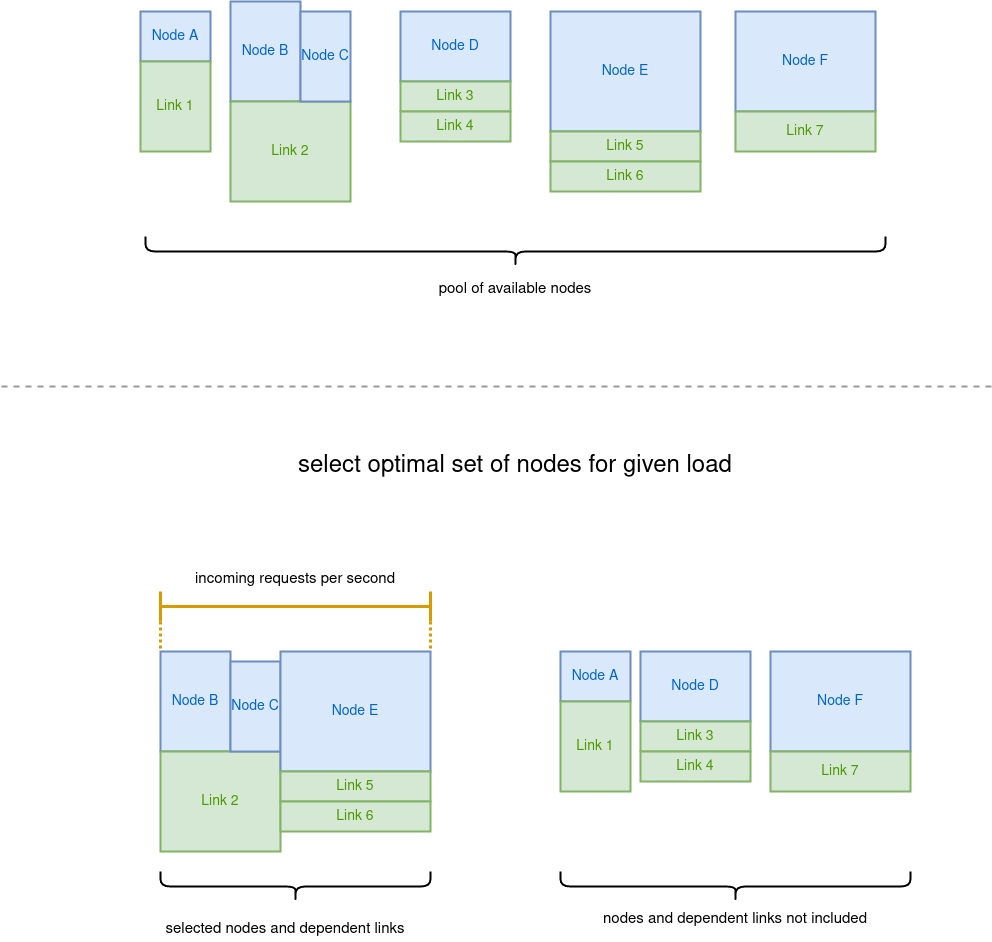
\includegraphics[width=14cm]{graphics/diagrams/lb_optimal_selection.png}
    \caption{Example visualization of an optimal selection of nodes, including their network links, for a given request load. Bounding boxes showing min/max load/performance, and fixed network latency performance parts are not displayed to keep the example simple.}
    \label{fig:lb_optimal_load}
\end{figure}

With this definition we can define the optimization problem an effective edge load balancer is trying to solve. The input to this problem is the given request load arriving from clients. In our visualization his corresponds to a set width. The objective is then to select nodes which when combined have the same width as the incoming client node, while at the same time maximizing the area of the nodes and network links selected. One needs to keep in mind that network links are not selected directly, but are implicitly included if selected nodes depend on them. Figure \ref{fig:lb_optimal_load} shows an example of such an optimal selection.

If the area is maximized in this optimization problem, response time is minimized, which is the goal a load balancer is trying to achieve.


While this visualization and problem is still relatively straightforward, there are other significant factors that we omitted until now:
\begin{enumerate}
    \item There are multiple functions, meaning that there are multiple "widths" or bins that need to be filled
    \item Functions share compute capabilities of nodes, meaning that performance regression, i.e. stretching and compression, needs to be considered over all functions running on a node
    \item Dependencies between network links and nodes aren't necessarily known
    \item Some network links necessarily handle traffic from outside the system, making performance regression assessment harder
    \item Actual performance profiles, i.e. dimensions, of nodes and functions aren't known
    \item Performance profiles, capabilities, client load, and function deployments change dynamically over time
\end{enumerate}

Considering these factors, load balancing in this context is a much higher-dimensional and thus more complex problem, where it is intuitively not clear whether an optimal solution is possible or if explicitly pursuing it in practise is even computationally feasible.


Since the true performance and regression characteristics of the nodes and network links are unknown, a load balancing solution needs to consider how this lack of information can be addressed. 
The simplest way to gather this information is by sending requests to nodes and observing response times. While this can yield insight into performance characteristics, these observations are merely a statistical sample, making them at least somewhat prone to misinterpretation. Especially when it comes to more complex behaviours such as functions sharing compute resources of nodes, or multiple nodes sharing network links.

Depending on the goals of the load balancer there is a risk/reward dynamic at play when it comes to sending requests to nodes in order to learn more about their performance characteristics. On one hand this can lead to "discovering" nodes that offer high performance and are able to handle a large number of requests, but on the other hand it could also lead to poor performance for those very requests in case network or compute capabilities are sub par.
There is no single correct answer to this dilemma, since the efficacy of any given solution would depend on the specific goals and tolerances of the application in question. In case \glspl{sla} exist that stipulate a certain response time for a minimum percentage of requests the risks might outweigh potential rewards, while an application that is somewhat tolerant to a fraction of requests being slow might experience a great performance uplift overall.
For our approach we consider \glspl{sla} to be out of scope, and therefore do not further address ways to address them. At the same time we want to point out that these are potentially relevant aspects for bringing serverless edge computing towards production readiness in the industry, and therefore highlight the areas where further study is needed.

\begin{figure}
    \centering
    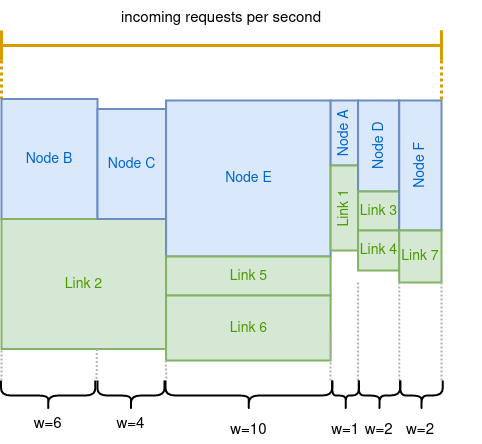
\includegraphics[width=10cm]{graphics/diagrams/lb_weights.png}
    \caption{Our approach as seen through the described visualization. All nodes are included in the "solution", and their load is determined by the load balancer assigning weights}
    \label{fig:lb_weights}
\end{figure}

Considering the myriad of potentially complicating factors for load balancing, in particular if one were to attempt to directly model the problem algorithmically, we decided to take a comparatively simple approach for our load balancing method.
In our approach we base our load balancing decisions solely on the total response time as it is observed by the load balancer. This means that we do not differentiate between times incurred from \gls{fet} and the times incurred from the networking portion. In this way we treat the total response time as a \textit{black box metric} to the overall system.
Our approach is to always include every single node in the "solution" to selecting appropriate nodes for the given width. This means that over the long term our approach gathers information about every potential node for every function replica that gets requested.
The disadvantage of this approach is that it dispatches requests to nodes that would not be included in a mathematically optimal solution, meaning that is will never reach the optimal performance possible assuming perfect knowledge of the system.
To counteract the performance penalty of including all nodes in the solution we assign them weights based on the response time they achieve.
This allows the load balancer to strike a balance between gathering information about the performance of the nodes available to the cluster, and processing requests as fast as possible.
Figure \ref{fig:lb_weights} shows the view of our approach on the system as described in the visualization. Note that the networking portion is not present, as our approach only considers the total response time in relation to the node it was sent to. Our approach also views each function replica separately, meaning that joint performance degradation of co-located function replicas is not modeled explicitly, only implicitly via the degraded performance observable through total request response times on that node.

There are a number of important considerations about the practical realization of our approach, which we will discussed next.


\subsection{Implementation}
As was just outlined our approach uses the response time as a black box metric to get insights into the system, and thus make load balanced decisions based on that information.
Since this basic idea does not constitute a concrete and testable approach we need to define the implementation details.

A well-known and simple implementation of this idea is the \textit{least response time} method of load balancing.
In this approach the server with the lowest average response time gets chosen whenever a request needs to be processed.
While this certainly works in general there are a few issues with this approach when it comes to serverless edge computing.
First, this approach can be problematic when it comes to co-located functions, as the load is not distributed among upstreams equally.
This leads to the fastest node being selected until its performance degrades enough for the next best node to be chosen.
Since there is no coordination that ensures some kind of balance, other functions that happen to be deployed on that node could experience severely hampered performance unexpectedly.
Second, this method does not take into account that the performance of nodes is, at least at first, unknown, and that it can change. A node that generally performs exceptionally well could be permanently excluded if at one point, for a spurious reason, performance was poor. A naive least response time load balancer would then likely rotate between a small handful of nodes that at one point performed well, effectively ignoring potentially better solutions.
These reasons point to the need of a more sophisticated approach than a naive implementation of least response time load balancing.

\subsubsection{Metrics Collection}
As explained, in our approach the metric used for load balancing decisions is the response time, specifically the time it takes between the load balancer forwarding the request to the selected upstream, and the load balancer receiving the response to the request.

Based on the response time data there are a number of performance metrics that could be calculated. Since our goal is to reduce the average total response time, we also chose the average response time as the key metric for load balancing decisions.
Depending on the requirements the load balancer needs to fulfill, other metrics could be used. A load balancer that is supposed to ensure a type of \gls{sla} might, for example, benefit from a percentile based metric instead.

In addition to effectively summarizing the performance of nodes, the metric needs to be time sensitive. Considering the performance of nodes can change over time, more recent values are more important as an indication of performance than those that lie farther back.
To address this, our approach makes use of a moving average with fixed window size.
We chose to use an exponential moving average since it has a number of advantages over more typical implementations.


\[\text{Given the previous average value } \mathbf{\bar{r}_{0}}\text{, the most recent response time } \mathbf{r}{,}\]
\[\text{the time passed since the last request }\mathbf{\Delta t} \text{, and the window size }\mathbf{w}\]
\[\text{The new average value }\mathbf{\bar{r}_{1}} \text{ is}\]
\[\bar{r}_{1} = (1 - e^{\frac{-\Delta t}{w}}) \cdot r + e^{\frac{-\Delta t}{w}} \cdot \bar{r}_{0}\]

The most significant advantage of this implementation over ones that use a buffer or a similar data structure, is precisely that complex data structures are not required. For each upstream only two values need to be recorded:
\begin{enumerate}
    \item The time the moving average was last updated
    \item The current value of the moving average itself
\end{enumerate}
While there are situations, where this can be less accurate, it is far easier to implement than buffer based solutions, since with these the required buffer size is unknown thus leading to frequent memory allocations and de-allocations.
Using an exponential moving average ensures minimal memory consumption, while at the same time being easy to understand and implement.

\subsubsection{Choosing Upstreams}
With the metrics collected what remains is deciding on upstreams based on those values. As previously outlined, naively choosing the upstream with the lowest average response time is potentially problematic.
For this reason our approach uses weighted round robin to decide which upstream should service a given request, where the response time metrics determine the weight assigned to each upstream.

The decision how exactly this weighted round robin gets implemented is surprisingly important, since the load balancing decisions affect the accuracy and volume of performance data gathered on each node, thus creating a feedback cycle that can, depending on the situation, lead to sub optimal performance.
For our approach we decided to use the same method employed by NGINX\cite{nginx}, a popular web-server and request proxy.
We chose this approach after experimenting with other solutions, and analyzing their performance profiles and characteristics with regard to the unique challenges posed by serverless edge computing environments.
Compared to other approaches is has the advantage of being deterministic, leading to all nodes being chosen eventually, which gives the load balancer sufficient data to make informed decisions, while at the same time distributing traffic in a mixed fashion between upstreams of different weights.
The evaluation methodology and experiment results of these experiments can be found alongside the general evaluation in the subsequent chapters.

\begin{algorithm}
  \KwIn{Set of available nodes $n_{0},n_{1},n_{...} \in N$}
  \KwIn{Weights for each of the nodes $w_{n_{0}}, w_{n_{1}}, ... \in W$}
  \KwIn{Current counter value for each node. $c_{n_{0}}, c_{n_{0}}, ... \in C$}
  \KwOut{The node the next request should go to}
    \For{$n \in N$}
    {
        $c_{n} \leftarrow c_{n} + w_{n}$ \Comment{add node weight to its counter}
    }
    $\text{selectedNode} \leftarrow n: c_{n} = max\{c: c \in C\}$ \Comment{select node with highest counter value}\\
    $c_{\text{selectedNode}} \leftarrow c_{\text{selectedNode}} - \sum_{w \in W}w$\\
    
  \Return{selectedNode}

  \caption{Smooth Weighted Round Robin}
  \label{alg:smooth-wrr}
\end{algorithm}
%todo: maybe rework this to be a bit more elegant
% currently a bit too much of a mashup between, math, set theory, code

\begin{table}[]
\centering
\begin{tabular}{llll}
Node          & \textbf{A}                & \textbf{B}                & \textbf{C}                \\
Weight        & \textbf{4}                & \textbf{2}                & \textbf{1}                \\ \hline
Iteration \#1 & \cellcolor[HTML]{FFCE93}4 & 2                         & 1                         \\
              & -3                        & 2                         & 1                         \\ \hline
Iteration \#2 & 1                         & \cellcolor[HTML]{FFCE93}4 & 2                         \\
              & 1                         & -3                        & 2                         \\ \hline
Iteration \#3 & \cellcolor[HTML]{FFCE93}5 & -1                        & 3                         \\
              & -2                        & -1                        & 3                         \\ \hline
Iteration \#4 & 2                         & 1                         & \cellcolor[HTML]{FFCE93}4 \\
              & 2                         & 1                         & -3                        \\ \hline
Iteration \#5 & \cellcolor[HTML]{FFCE93}6 & 3                         & -2                        \\
              & -1                        & 3                         & -2                        \\ \hline
Iteration \#6 & 3                         & \cellcolor[HTML]{FFCE93}5 & -1                        \\
              & 3                         & -2                        & -1                        \\ \hline
Iteration \#7 & \cellcolor[HTML]{FFCE93}7 & 0                         & 0                         \\
              & 0                         & 0                         & 0                        
\end{tabular}
\caption{An example of weighted round robin iteration results when using Algorithm \ref{alg:smooth-wrr} as we do in our approach. Colored cells indicate the selected node at the iteration.}
\label{tab:smooth-wrr-demo}
\end{table}

Algorithm \ref{alg:smooth-wrr} shows a pseudo-code implementation of our weighted round robin component using the approach also used in the NGINX source code \cite{nginx-wrr}.
Table \ref{tab:smooth-wrr-demo} shows how this implementation of weighted round robin distributes requests between upstreams of different weights. Note that the proportions between the weights are considered when choosing upstreams without using a fixed ordering based on weight, meaning that choices of upstreams with lower weights are interleaved between choices of upstreams with higher weights. %todo rewrite this. It's super unclear what is meant by this.

The only part of our load balancing approach that is not yet described is how the average response time recorded is mapped to the weight used by our weighted round robin implementation.
There are a number of ways in which values like this can get mapped to weights.
There is, unfortunately, no single correct answer since the lack of precise information on the state and performance of nodes and the network prevents us from reliably making globally optimal load balancing decisions.
There are two factors that determine how response times are mapped to weights:
\begin{enumerate}
    \item The weight range response times should be mapped to
    \item The function by which they are mapped to these weights
\end{enumerate}

In our approach we chose to use a fixed range of weights, since this makes sure every upstream is assigned at least a fixed fraction of traffic.
This guarantees that the response times of all upstreams are sampled eventually, preventing a situation where a significant change in the performance of an upstream goes unnoticed forever.
The weight of each upstream is determined by it's average response time in the last value and calculated using the following formula:
\[ \text{Let } \bar{r} \in R \text{ be the set of response time averages, and }\]
\[ w_{\text{min}} \text{ the minimum weight, } w_{\text{max}} \text{ the maximum weight, then}\]
\[ \text{the weight for each response time average } w(\bar{r})\text{ is defined as}\]
\[ w(\bar{r}) = max\{w_{\text{min}}, \frac{w_{\text{max}}}{(\frac{\bar{r}}{min\{\bar{r}: \bar{r} \in R\}})^{s}}\} \]
\[ \text{where } s > 0\text{ is a chosen scaling factor }\]

The scaling factor determines how weights correlate to response time. A scaling factor of 1 means that there is a linear relationship between the average performance and the weight.
Figure \ref{fig:weight_mapping_example} shows the effect different scaling factors have on weight mappings in the weight range of 1-10. Both continuous and integer values are shown, since it depends on the weighted round robin implementation which of the two can be used.
Based on grid-search experiments we chose a weight range of 1-25, and a scaling factor of 2. (//note to me: these experiments should be expanded a bit and values updated if necessary).
The experiments that determined this choice will be described in detail in subsequent chapters.

% idea: factor (i.e. deciding on linearity) depends on how strong the link between performance and capacity is. i.e. if strong performance means high capacity, we can assign super high relative weights. Is this even important? Since on paper overload etc. should eventually lead to a balance being achieved, no?
% idea: spread (i.e. size of weight range) depends on how dynamic the system is and how high we value information gain, since high spread -> more optimal in static condition. low spread -> discovers changes faster in dynamic conditions.

\begin{figure}
    \centering
    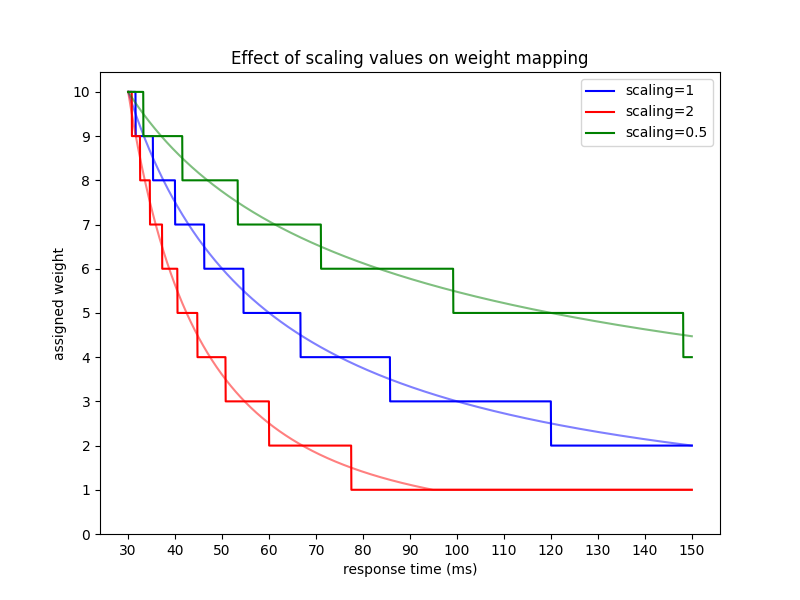
\includegraphics[width=10cm]{graphics/graphs/weight_mapping_scaling_example.png}
    \caption{Plot showing the effects of different scaling factors on how response time averages are mapped to weights.}
    \label{fig:weight_mapping_example}
\end{figure}


\subsubsection{Framework Integration}
In our approach the load balancers are assumed to be integrated into the serverless framework.
This means that load balancers are notified of changes to function replicas, meaning that they are always aware which functions exist, and which exact replicas are available for each function.
From a practical perspective this is simple to achieve in a production implementation as serverless frameworks already provide this information in some way, and the underlying technologies, typically some kind of container orchestration, also have means to retrieve the necessary data.

Apart from the available functions and their respective replicas, new load balancer instances are initialized with response time values and weights of already running load balancer instances nearby.
While the load balancer still needs to adapt its weights based on its specific client load and position in the network, this initial pre-loading of values allows it to converge on a stable configuration faster, thus resulting in quicker performance gains.


% Target: 8 pages with figures
\section{Osmotic Scaling and Scheduling}
In this section we describe our approach to scaling, and scheduling load balancer replicas, meaning the process by which we decide how many load balancer instances are in the system, and on which nodes they are placed.

\subsection{Osmotic scaler and scheduler}
To determine the number of replicas and their location we opted for an approach based on \textit{osmotic pressure}.
Like we outlined in previous chapters, osmotic pressure is a high level concept supposed to facilitate elastic diffusion, elastic diffusion being the process by which a central starting configuration, typically in the cloud, is extended to the edge dynamically based on request load with the goal of providing low latency communication for edge clients\cite{osmotic-middleware-rausch}. 
The general idea of this approach is that client requests generate pressure on nodes that are close to the clients, meaning that they could potentially host a load balancer instance, and then using this pressure in conjunction with a set threshold to determine both the number of load balancer instances and their locations.
If pressure at a node exceeds a certain level, because there are a lot of client requests originating close by, a load balancer will the, be placed at the node, thus lowering the pressure.
Conceptually this approach is supposed to create an equilibrium of pressure throughout the system, which results in a well-chosen set of load balancer instances.
This means that by using an osmotic approach, the scaling and scheduling decisions are effectively made together and cannot be controlled separately.

The main challenge of realizing an approach based on the concept of osmotic pressure is finding the method by which pressure is calculated. This can be particularly challenging when the system requires a manually set pressure threshold, since this requires the threshold value to fulfill a number of criteria:
\begin{enumerate}
    \item \textbf{Intuitive:} the threshold value should be at least somewhat intuitive to whoever determines it. It should be clear what a certain pressure threshold \textit{means}, and how it will affect the system.
    \item \textbf{Robustness:} the threshold should be reasonably robust to dynamically changing systems. A few extreme outliers in the system, for example extremely far or close nodes, should not require the threshold to be changed to still achieve the desired behaviour.
    \item \textbf{Linearity:} while not necessarily fully achievable, ideally changes in the threshold value should have a close to linear relationship with the scaling and scheduling behaviour. This is important in conjunction with its intuitiveness and is important to prevent sudden, unexpected effects such as dramatically changed system behaviour with minuscule changes in the threshold value.
\end{enumerate}

\subsection{Calculating osmotic pressure}
Building on the previously outlined requirements we can develop a pressure calculation methodology.
\subsubsection{Required data}
Because osmotic pressure based scaling and scheduling is at its core still a heuristic-driven approach, we cannot assume to have perfect global knowledge of the system.
Our approach is built with that in mind, staying close to assumptions about data availability already used for the load balancers themselves, and building on information current container orchestration platforms such as Kubernetes already provide.
For our calculation of osmotic pressure we require the following data:
\begin{itemize}
    \item Network locations of all function replicas, i.e. which nodes the instances are running on
    \item Network locations of all clients
    \item Number of all client requests, and which functions they are for
    \item Network locations of all load balancer replicas
    \item Network distances (latency) between nodes and clients
\end{itemize}
Replica information is readily available through state of the art container orchestration platforms, while network distances and exact client request numbers are relatively simple to obtain.
Because of this comparatively available set of data, we believe that our approach could easily be integrated into current serverless frameworks.
\subsubsection{Concept}
The basis of our pressure calculation is a hypothetical "what-if" scenario.
For all nodes in the system that could potentially host a load balancer, and are currently not doing so, we ask the question "what if there was a load balancer instance running on that node".
We then compare this hypothetical scenario to the current state of the system and determine whether the hypothetical addition of the load balancer on the node would constitute an improvement or deterioration in performance, and if so by how much.
For nodes that are hosting a load balancer already we do the same in reverse and ask "what if there wasn't a load balancer there", once again estimating whether performance would improve or deteriorate.

The two metrics we use to determine the impact of adding or removing load balancer replicas are the \textit{request share} and the \textbf{projected performance} of the node.
These metrics are calculated for each node on a per-function basis, and ultimately determine the pressure.

\subsubsection{Request Share}
\begin{figure}
    \centering
    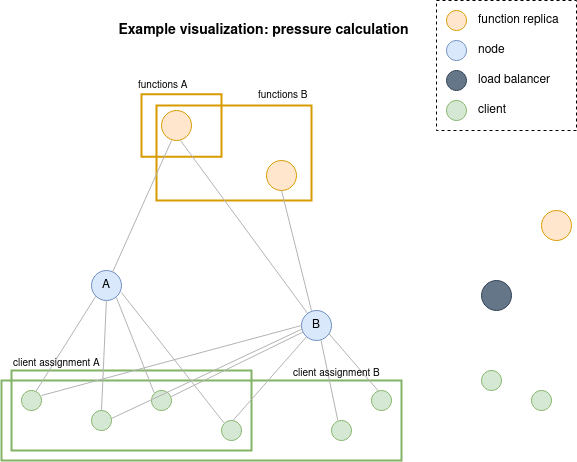
\includegraphics[width=12cm]{graphics/diagrams/client_lb_assignment.png}
    \caption{Assignment of clients and function replicas to potential load balancer nodes during pressure calculation}
    \label{fig:cl_lb_assignment}
\end{figure}
The request share is one of the central metrics we use to determine a node's pressure. In principle it shows which portion of the system's total incoming requests would be routed over that node, if it had a load balancer.
To calculate this value we need to first look at client assignment, meaning the process by which it is determined which client will send requests to which load balancer.

As we already outlined previously, one of our core assumptions is that clients will send their requests to whichever load balancer is closest from a network perspective, which is the load balancer with the shortest \gls{rtt}.
In keeping with our hypothetical scenario of "what if there was a load balancer on this node", clients will send their requests to this potential new load balancer if that node is closer to the clients than whichever load balancer instance is currently closest.
An example visualization of this client assignment for calculating request share can be seen in Figure \ref{fig:cl_lb_assignment}.
The specific number of clients our potential load balancer would service is, however, only of secondary importance. The more important and precise metric is the number of requests it will service.
We do not really care about whether there are a lot of clients sending few requests, or a low number of clients sending a large amount. What is important is only the number of requests going to the potential load balancer relative to the total amount sent.
Generally the data for this calculation is readily available, and can easily be gathered for example via existing load balancers reporting on the requests they receive.

A point to note here is that we only consider the requests sent within a certain time frame for this calculations, as they should be recent enough to be relevant for current scaling and scheduling decisions.
In our case we chose this time frame to be the last 60 seconds, which is relatively short but works within the relatively dynamic and heterogeneous systems we consider.
For real deployments this value might have to be adapted based on how dynamically the request load changes, how many requests each client typically sends in a session, and what amount of load is generally typical of the system.
The important point to consider here is that the time frame needs to be long enough to give a reasonably accurate picture, while not being so long that the data is delivers is not reflecting the current state of the system anymore.

Lastly, since there are multiple functions in the system, which we generally consider to be of equal importance, we calculate the request share the potential load balancer would receive on a per-function basis.
Thus we define the \textit{request share} as the following:
\[ \text{Let }N\text{ be the set of nodes,} \]
\[ L\text{ the set of nodes with running load balancer instances,} \]
\[ F\text{ the set of serverless functions,} \]
\[ \text{and }C\text{ the set of clients.} \]
\[ \text{Further let } dist(n,c) \text{ be the distance between a node } n \in N \text{ and client }c \in C\text{,}\]
\[ \text{ and let }requests(c, f) \text{ be the number of requests from client }c \in C \text{ for function }f \in F\]
\[ \text{Then for each node }n \in N\text{ the assigned clients are defined as} \]
\[ assignment(n) = \{c | c \in C \land dist(c,n) < min\{dist(l, c) | l \in L\}\}\]
\[ \text{Finally the request share for node } n \in N \text{ for function }f \in F \text{ is defined as } \]
\[ rqshare(n,f) = \frac{\sum_{c \in assignment(n)}requests(c,f)}{\sum_{c \in C}requests(c,f)}\]
Thus we define the request share of a node for a given function, as the fraction of all requests for that function the node would receive if it had a load balancer instance running.
\subsubsection{Projected Performance}
The second major metric that determines the pressure of a given node is what we refer to as the \textit{projected performance}.
This metric is once again based on the hypothetical scenario of "what if there was a load balancer on the given node" and is supposed to estimate the level of network performance we could expect if a load balancer is actually placed there.
Conceptually our notion of performance is rather simple.
It is determined by how close the clients are that would be assigned to that node, and by how close the function replicas are.
We once again calculate this metric for each node, and on a per-function basis.
To calculate the \textit{client distance} we use the average distance of all assigned clients, weighted by their relative share of requests among the assigned clients for the given function.

The calculation of the \textit{function distance} is somewhat more intricate.
Using a flat average over all function replicas is not a particularly suitable metric, since this would also consider the distance of function replicas that are far away, meaning that we would include the distance to function replicas we don't want the requests being sent to in the first place.
To address this issue we only consider a subsection of function replicas to calculate the function distance.
Our approach to the function distance is based on the assumption that the function scaling component correctly scales the function as required, meaning that we assume that the total number of function replicas is sufficient to serve the given number of incoming requests.
The number of function replicas we consider for a node is based on that nodes request share. We take into account the fraction of closest function replicas equal to the request share of the node for which we want to calculate the function distance.
If a node, for example, has a request share of 0.5, meaning 50\%, then its function distance is the average distance of the 50\% closest function replicas.
An example of this can once again be seen in Figure \ref{fig:cl_lb_assignment}, where nodes A and B have a differently sized share of functions assigned to them for distance calculation based on their respective request share.
Since we assume that the function replica scale is sufficient to handle the systems requests, this should mean that, not accounting for heterogeneity in function replica performance, the replicas considered for the function closeness metric are sufficient the incoming requests of the load balancer.
The reason we are not considering heterogeneity in replica performance is that this factor is not known beforehand, and in addition hard to estimate.
Finally we add the function distance and client distance together and invert them, since our subsequent calculations require the projected performance metric to have high values indicating good performance, and low values indicating poor performance.
Making this explicit we arrive at the following formulation for our projected performance:
\[\text{Let } replicas(f) \text{ be the set of replicas of a function }f \in F\]
\[\text{Then the client distance for a function }f \in F \text{ and node }n \in N \text{ is}\]
\[cldist(n,f) = \frac{\sum_{c \in assignment(n)}dist(n,c) \cdot requests(c,f)}{\sum_{c \in assignment(n)}requests(c,f)} \]
\[\text{Let }repdist_{n,f} = \langle r_{0}, r_{1}, ... \rangle \text{ be the list of replicas for a function }f \in F \text{ ordered by} \]
\[\text{their distance to }n \in N \text{ in ascending order such that for each pair } \]
\[(r_{i},r_{j}) \in repdist_{n,f}^{2}: i < j \implies dist(n, r_{i}) \leq dist(n, r_{j})\]
\[\text{Then the set of replicas considered is } \]
\[replicas(n,f) = \{r_{i} | r_{i} \in repdist_{n,f} \land i < \lfloor rqshare(n,f) \cdot |repdist_{n,r}| \rfloor\}\]
\[\text{Thus the function distance is }fndist(n,f) = \frac{\sum_{r \in replicas(n,f)}dist(n,f)}{|replicas(n,f)|} \]
\[\text{Finally the projected performance is }perf(n,f) = \frac{1}{cldist(n,f) + fndist(n,f)} \]
Needless to say slight adaptations of these formulas are necessary for a practical implementation.
For our simulator based evaluation the formulas are used exactly as we present them here, with the exception that special values are used as placeholders for undefined values, particularly those that result from a division by 0.
If a node has a request share of 0 for example, the projected performance is simply set to 0.
Likewise if the request share is > 0, the function distance calculation will take into account at least one replica, even if based on these formulas none would qualify.


\subsubsection{Pressure}
Now that we defined request shares and the projected performance we can move on to the actual pressure calculation.
In our approach we calculate what we call \textit{relative pressure}.
This means that the pressure of a given node is always in relation to the current state of the system, and not in absolutes.
This is done to ensure that the pressure calculation is not dependent on a-priori knowledge of the system.
If, for example, pressure were directly related to the number of requests per second the user would have to define what number of requests is considered high or low manually beforehand, negating precisely the kinds of advantage serverless frameworks are supposed to afford: Alleviating developers from complex configuration.

Our proposed notion of pressure is focused on the changes adding a load balancer on the node in question would bring to the system.
We start out by making an estimation of the average performance and impact of a load balancer in the system.
This notion of performance is based on the already described projected performance, and the load balancers request share.
We cannot rely purely on the projected performance, as it is also tremendously important for how many requests this performance is provided.
If we, for example, have a situation where we need to decide between two nodes which could potentially host a load balancer, that have a very high projected performance, then we most likely improve overall system performance more by selecting the node with the higher request share, since the high expected performance will affect more requests.

We call our estimation of the current system performance the \textit{status quo performance}.
To calculate it we once again rely on the projected performance, and the request share of node, although since we are interested in the current state of the system we consider these metrics only for nodes which currently host a load balancer.
The calculation of these metrics is exactly the same as for nodes that do not have load balancer instances deployed on them.
A slight difference to note is that the partition of clients onto nodes with load balancers will be without overlap, meaning that if we sum up all the request shares of a function over all nodes with a load balancer, the result would be 1, i.e. 100\%.

For our pressure metric this status quo performance is calculated using a weighted quantile.
The projected performance of the load balancer nodes are the values over which the quantile is calculated, while their respective request share is the weight.
We use the 50\% weighted quantile, also referred to as the weighted median, as our status quo performance.
In our testing the weighted median provided a robust metric that behaved predictably and similarly over different network topologies and cluster sizes.
It is, however, conceivable that there are situations in which this quantile should be set higher or lower depending on how dynamic the system changes, and how heterogeneous its structure and network topology are.
We should also note that at this point all of these metrics are still calculated on a per-function basis.
The values for each function are only combined at the very end, weighted by how important the individual functions are.
In our case the importance of individual functions is determined by which proportion of total requests are directed to it.
This means that we effectively treat each request as equally important and thus a function which gets double the traffic of another, for example, would also be considered twice as important when the individual function based metrics are combined.

% todo this should probably we rewritten a bit to be less repetitive
With this metric we can now calculate our pressure metric. For a given node we do this by calculating its impact on the system compared to the status quo performance.
Assuming that the status quo performance represents the current system performance overall, we compare the status quo performance with the performance of the system with the node added.
Since, as described earlier, the current set of load balancers services all client requests, adding a new load balancer will remove some of the traffic from existing load balancers.
This amount is represented by the potential load balancer node's request share.
To then calculate the system performance with the potential load balancer added we replace a part the size of the node's request share with the nodes performance.
Lastly we compare by how much adding a load balancer on this node changes the overall system performance, by calculating their difference in percent.
This percentage difference is the pressure value we use to make scaling and scheduling decisions in our osmotic system.
A positive pressure indicates that adding would likely improve performance, while negative pressure indicates that it would likely deteriorate overall system performance.
Thus we formally define our pressure as follows:
\[\text{For each function }f \in F \text{ it's relative importance is }\]
\[importance(f) = \frac{\sum_{c \in C}requests(c,f)}{\sum_{f' \in F}\sum_{c \in C}requests(c,f')} \]
\[\text{Let the set of tuples of a load balancer node's performance and request} \]
\[ \text{share for a function }f \in F \text{ be} \]
\[lbperf_{f} = \{(perf(l,f), rqshare(l,f)) | l \in L\} \]
\[\text{Then for a function the weighted median performance is } statusquo(f) = weightedmedian(lbperf_{f})\]
\[\text{Based on this we can estimate the system performance when adding a load balancer on node }n \in N\]
\[ addperf(n,f) = (rqshare(n,f) * perf(n,f)) + ((1 - rqshare(n,f)) * statusquo(f))\]
\[\text{which relative to the status quo performance gives us the pressure per function} \]
\[ fp(n, f) = \frac{addperf(n,f) - statusquo(f)}{statusquo(f)}\]
\[\text{Then combined the final pressure of the node is } p(n) = \sum_{f \in F}fp(n,f) \cdot importance(f)\]

\subsubsection{Downscaling Pressure}
Just like we need pressure to determine where load balancers should be scheduled, we also need to decide on conditions which trigger an existing load balancer to be removed.
Without this mechanic the osmotic scaling and scheduling component would not be able to properly adapt to changing system conditions, since load balancers that aren't placed effectively anymore cannot be removed.
During development we learned that an important property of the osmotic scaling and scheduling system is that it is consistent.
For our purposes this means that it should find a stable configuration eventually that doesn't change anymore unless the surrounding system parameters change.
In our testing the use of the exact same metric for removing load balancers as for adding them led to oscillations in their scheduling, meaning that there were cases were a load balancer would be added only to be removed again immediately.

To address this we use a slightly different measure of pressure for removing load balancer replicas.
It is also based on a hypothetical scenario, though in this case we try to estimate the consequences removing a load balancer would have on the system performance.
Compared to the pressure when adding load balancer replicas, we use a somewhat more accurate measure than for the removal process, since the original and future state of the system are more well known, considering it relies on more tangible and less hypothetical data.
First, the status quo before removal is calculated.
This is a weighted average of the projected performance of all load balancers weighted by their request share.
For the system performance once the load balancer is removed, we calculate how the system structure would change if the load balancer is removed.
The primary change this entails is that the removed load balancers clients would then send their requests to the next closest load balancer instance.
For simplicity and calculation efficiency, we assume that the clients would be assigned to whichever load balancer is closest to the one potentially getting removed.
At this point we recalculate the projected performance and request share of the load balancer that takes over the clients.
Based on this we can then calculate the system performance with the load balancer removed by again using a weighted average over the projected load balancer performances weighted by their request share, with the difference being that the load balancer we potentially remove is no longer counted, and its clients are moved to the next closest load balancer.
We then have an estimation of system performance with and without the load balancer in question, and go on to calculate their percentage difference.
This percentage difference tells us by how much removing the load balancer would affect overall system performance in percent, and based on a user defined threshold the scaler then decides to remove or keep each individual load balancer instance.
\[\text{For a function }f \in F \text{ the pre-removal status quo system performance is }\]
\[rmstatusquo(f) = \sum_{l \in L}perf(l,f) \cdot rqshare(l,f)\]
\[\text{If we then remove a load balancer }l \in L \text{ the clients are taken over by another load balancer} \]
\[l': dist(l,l') \leq min\{dist(l,l'') | l'' \in L \setminus \{l\}\} \implies assignment(l') = assignment(l') \cup assignment(l)\]
\[\text{Giving us the adapted set of load balancers }L' = L \setminus \{l\} \]
\[\text{Then the system performance without the load balancer for a function is} \]
\[rmperf(l,f) = \sum_{l' \in L'}perf(l',f) \cdot rqshare(l',f) \]
\[\text{Based on which we can calculate the removal pressure per function as}\]
\[ rmfp(l,f) = \frac{rmperf(l,f) - rmstatusquo(f)}{rmstatusquo(f)}\]
\[\text{and then combine them to the final removal pressure } rmp(l) = \sum_{f \in F}rmfp(l,f) \cdot importance(f)\]

\subsubsection{Throttled Scaling}
In our approach the scaling and scheduling components calculates pressures for all nodes and load balancers, and then makes subsequent scaling decisions, at a fixed interval.
While in theory multiple nodes could have a pressure beyond the set threshold that warrants adding a load balancer in a single interval, in our approach we artificially throttle this amount.
In our implementation of the scaling and scheduling component only a single load balancer can be added or removed per iteration.
We compensate for this comparatively slow rate of change by running the scaling and scheduling calculations at relatively short intervals.
There are two major reasons for our choice to limit the rate of change in the system in this way.

\begin{enumerate}
    \item The pressure metrics and calculation are based on the addition or removal of a single instance
    \item Since request shares potentially overlap, scheduling multiple load balancers often leads to immediate removal during the next scaling and scheduling cycle
\end{enumerate}

During development we observed faster convergence to a stable configuration when only adding or removing a single load balancer at a time.
We also considered changing our pressure calculations to optimize for a faster rate of change, but decided against it because these calculation are much less intuitive, which is detrimental to the ease of parametrization of the system, and most importantly the computational effort rises sharply with the number of load balancer instances that are considered simultaneously.
While the single node calculations we use only require calculating a maximum of 250 scenarios for a system with 250 nodes, the equivalent calculations for two nodes being scheduled simultaneously would require calculating up to 31125 scenarios for an equally sized system.
While this does limit the potential rate of change, we believe that a rate of change of about 4 load balancers per minute, which could still be increased if necessary, should be enough to handle the requirements of even comparatively dynamic systems.



